\section{Approach}
\label{s:oldapproach}
%Approach; What selection of deep uncertainty methods are you using, in what order, and why? This should be clearly motivated and grounded in the literature

% Analysis is carried out across the explicated rival problem framings and relies on state-of- the-art deep uncertainty techniques
Multiple alternative approaches were considered to analyse the explicated problem framings, with a description of some alternative considerations described in the Appendix (MAYBE??). Ultimately, a straightforward combination of techniques were adopted to analyse and interpret the problem framings of Gorssel, as well as it's two rival/coalition-forming actors, Deventer and Overijssel.

%In what order are we using the tools and why are we using them this way
We have opted to combine multi scenario multi-objective robust decision making (multi-scenario MORDM) and dynamic adaptive policy pathways (DAPP) in our approach to perform risk assessment. DAPP allows for a lot of flexibility, as it represents sequences of promising alternative ways for Gorssel to achieve their objectives as described in Section~\ref{s:prob_frame} \citep{Walker2013}. Multi-scenario MORDM allows us to asses the uncertainty within the variables and analyse their implications. An adaptation tipping point is the point at which a policy does no longer meet the criteria (\textbf{CITE: Kwakkel 2016 paper from week 8 readings)}.

We employed TU Delft's open source EMA workbench library which allows for simulations, visualisation and analysis in Python \parencite{kwakkel_exploratory_2017}. An adapted version of the model presented in \citetitle{ciullo_accounting_2019} was used to discover possible strategies. And the tool of Deltares was used to create the metromap. The workflow is shown in Figure~\ref{fig:flowchart} and discussed in detail in the sections below.

\begin{longtable}[c]{p{2cm}p{2cm}p{5cm}l}
\caption{Selected criteria, adaptation objectives, metrics and tolerable impacts}
\label{tab:criteria}\\
\textbf{Criteria}        & \textbf{Adaptation Objective} & \textbf{Metric}                                           & \textbf{Tolerable impact} \\
\hline
\endfirsthead
%
\endhead
%
Land encroachment & TBD & Expected Annual Damage Gorssel & TBD \\
Difference in flood risk & TBD & Difference Expected Number of Deaths Deventer and Gorssel & TBD\\
Difference in protection & TBD & Difference Expected Annual Damage Deventer and Gorssel & TBD
\end{longtable}


\subsection{Generation of scenarios}
Generate the uncertainty space: Generate n number of cases with LHS that incorporate the uncertainties (and store them in a csv file). Alternatively we could use optimisation as well for this.

\subsection{Below for each policy + for base case (without policy) (so iteratively)}
\subsubsection{Identification of adaptation tipping points}
Use scenario discovery (PRIM - so subspace partitioning)) to search the results to identify adaptation tipping points. So the results of PRIM are those boxes (which are interesting clusters that contain the interesting cases). (So when we provide PRIM the threshold for outcome, and it will give us the ranges in uncertainty - our triggers).

\subsubsection{Scenario selection}
This was part of ass 9. We should be fine.

\subsubsection{Generation of policies: Directed search to get candidate solutions (policies)}
Generate decision space: GET THEM POLICIES
(So we get the Pareto-approximate set of solutions)

%Z: Don't think I agree. Moro sounds overkill and is perhaps therefore not the best choice. So the choice is between MORDM, Multi-scenario MORDM and normal RDM, and on top of that, they're all frameworks (meaning we might need to change our methodology depending on which one we choose). I think Bartholomew_2020 (week 7) is more informative. So the current workflow is pretty much just RDM, with MORDM we'd need to change some stuff since we need to pick a reference scenario, and with Multi-scenario MORDM we don't need to pick a reference scenario. In the paper from Kwakkel + Eker they talk more about Multi-scenario MORDM. It's prettty much just running MORDM a couple of times + some additional steps. (If we have the time we could adapt our method to multi-scenario MORDM, but I don't think we'll have the time, so maybe stick with RDM?) $
%No you're right, it is probably way too much overkill to go with MORO. 
%Ok I am going to include a multi-scenario MORDM version right now

\subsubsection{Sensitivity analysis}
assess the policies (Sobol, extra trees, Morris) (so we stress test the found candidates) - so with the parcoords plots and stuffffz
%I found my reasoning again, I thought extra-trees as Rozen2018 describes that it is computationally less expensive than Morris, but approximates the sobol relative importance effects. 

Have a selection of policies (candidate solutions) then test how these behave for different actor's problem framings (sensitivity analysis).

\subsubsection{Update adaptation pathway}
(so just update it with the new tipping point + policies)

\begin{figure}[h!]
    \centering
    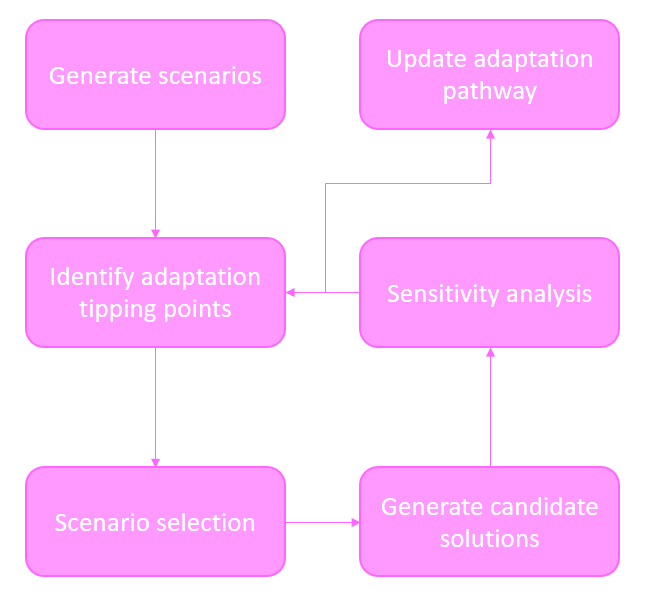
\includegraphics[width=0.45\textwidth]{report/figures/flowchart.png} 
    \caption{Flowchart}
    \label{fig:flowchart}
\end{figure}



%NSGAII-Epsilon - most it can handle is 7-8 objectives. Therefore, the objectives were prioritised.
%Z: to be fair, this is probably also easiest to communicate to the client, lol

%Scenario discovery (PRIM)

%Directed search(MOEA, MORDM, multi-scenario MORDM, MOE, may need scen disco) $\xrightarrow{}$ sensitivity analysis (Sobol, MOrris, Extra-Trees) $\xrightarrow{}$ Test on found scenarios

%Tools used are unique from policy presentation - you can use MORDM and do policy pathways - CITE: Kwakkel, Haasnoot and Walker, 2015

% Robustness metrics: Key takeaway from McPhail - you should use at least 2 robustness metrics, one satisficing and one regret-based.



\subsection{Lisettes brainstorm session}
\begin{itemize}
    \item problem formulation: levers + uncertainties for all actors
    \item gen scen: randomise scenfor Gelderland
    \item preprocessing: normalization + pca (+possibly pca\_preprocessing)
    \item Scary events: identify \textbf{not adaptation tipping point} but signposts \& triggers Gorssel should be watching out for with events for Gelderland shit 80\% bad scenarios 20\% everything else Pareto Principle 
    \item Use multi-scenario MORDM on the scenarios we select from previous step that to find out what policies work best against \underline{all of those scenarios} that that FIT our robustness criteria
    \item sensitivity analysis on these policies.
    \item Irenes paper: https://agupubs.onlinelibrary.wiley.com/doi/full/10.1002/2017WR020524  they derive the pareto optimal set for each rival framing -> our first diagnostic verification step is to reevaluate the solutions from each of the problem formulations in the objective spaces of all of the other formulations (so they optimise again)
\end{itemize}

FOr generating scenarios obviously LHS
Sensitvity analysis: Luka recommended extra-trees
ALTERNATIVELY:

Bad policies: We can perform directed search over the decision levers to find out what policies are the worst for Gorssel (with MOEA), and need to be prevented. We can include an argument to calculate the distance from a certain threshold as well (for both uncertainties and outcomes). We also do not need to do this for all decision levers (like obviously not our own).

Perform experiments can apparently be done with sampling over levers.

\begin{figure}[h!]
    \centering
    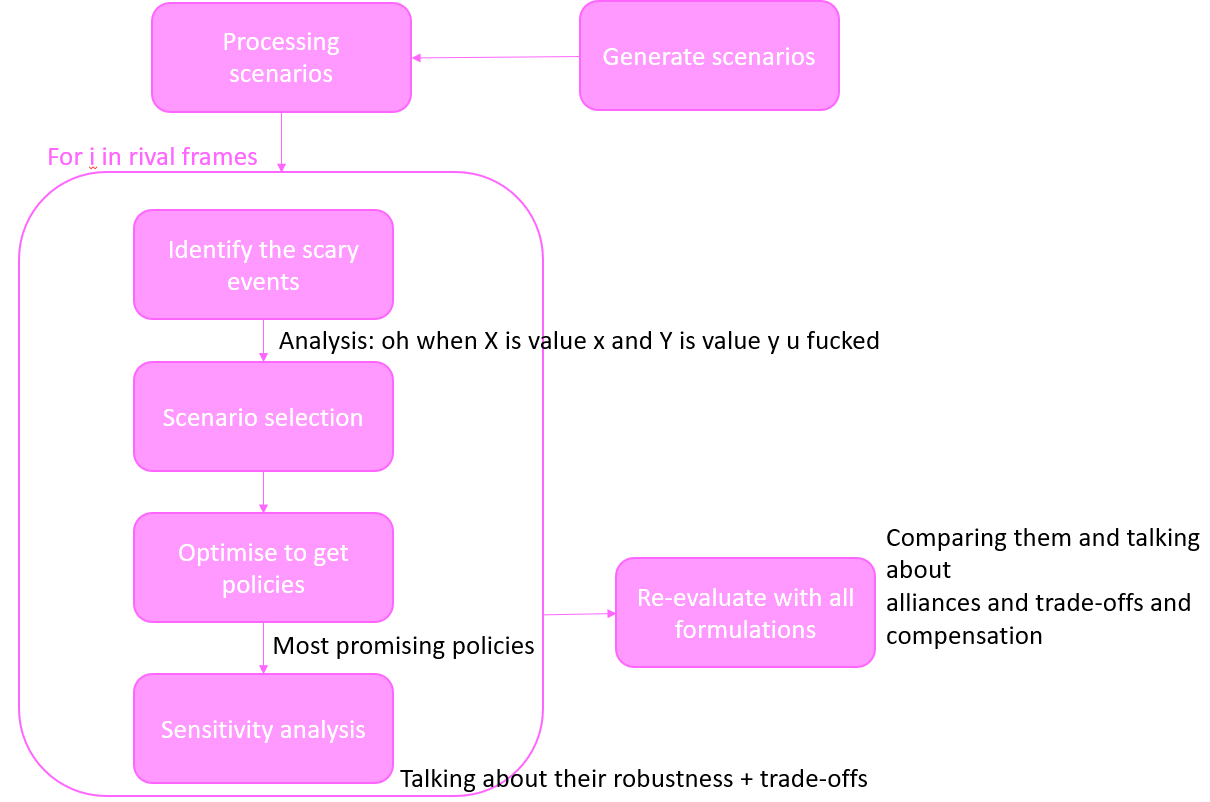
\includegraphics[width=0.6\textwidth]{report/figures/methodology.png} 
    \caption{Methodology}
    \label{fig:methodology}
\end{figure}

